% ============================================================
% Question Bank: ch04-04 Factoring Expressions
% Topic Title: Factoring Expressions
% CCSS: 7.EE.A.1
% Questions: 27 (15 MC + 6 SA + 6 Graphical)
% ============================================================

% --- Multiple Choice Questions (15) ---

\begin{practiceQuestion}{4-4-q01}{mc}
\begin{questionText}
What is the greatest common factor (GCF) of $16$ and $24$?
\end{questionText}
\choiceA{$4$}
\choiceB{$6$}
\choiceC{$8$}
\choiceD{$12$}
\correctAnswer{C}
\explanation{Factors of $16$: $1, 2, 4, 8, 16$. Factors of $24$: $1, 2, 3, 4, 6, 8, 12, 24$. The greatest common factor is $8$.}
\end{practiceQuestion}

\begin{practiceQuestion}{4-4-q02}{mc}
\begin{questionText}
Factor $8x + 20$.
\end{questionText}
\choiceA{$2(4x + 10)$}
\choiceB{$4(2x + 5)$}
\choiceC{$8(x + 20)$}
\choiceD{$4(2x + 20)$}
\correctAnswer{B}
\explanation{GCF of $8$ and $20$ is $4$. Factor: $8x \div 4 = 2x$ and $20 \div 4 = 5$. Result: $4(2x + 5)$.}
\end{practiceQuestion}

\begin{practiceQuestion}{4-4-q03}{mc}
\begin{questionText}
Factor $18a - 12$.
\end{questionText}
\choiceA{$6(3a - 2)$}
\choiceB{$3(6a - 4)$}
\choiceC{$2(9a - 6)$}
\choiceD{$6(3a + 2)$}
\correctAnswer{A}
\explanation{GCF of $18$ and $12$ is $6$. Factor: $18a \div 6 = 3a$ and $-12 \div 6 = -2$. Result: $6(3a - 2)$.}
\end{practiceQuestion}

\begin{practiceQuestion}{4-4-q04}{mc}
\begin{questionText}
Which is the completely factored form of $12m + 18$?
\end{questionText}
\choiceA{$2(6m + 9)$}
\choiceB{$3(4m + 6)$}
\choiceC{$6(2m + 3)$}
\choiceD{$12(m + 18)$}
\correctAnswer{C}
\explanation{GCF of $12$ and $18$ is $6$. Factor: $12m \div 6 = 2m$ and $18 \div 6 = 3$. Result: $6(2m + 3)$. Choices A and B do not use the GCF.}
\end{practiceQuestion}

\begin{practiceQuestion}{4-4-q05}{mc}
\begin{questionText}
Factor $21x + 35y$.
\end{questionText}
\choiceA{$3(7x + 35y)$}
\choiceB{$7(3x + 5y)$}
\choiceC{$7(3x + 35y)$}
\choiceD{$21(x + 5y)$}
\correctAnswer{B}
\explanation{GCF of $21$ and $35$ is $7$. Factor: $21x \div 7 = 3x$ and $35y \div 7 = 5y$. Result: $7(3x + 5y)$.}
\end{practiceQuestion}

\begin{practiceQuestion}{4-4-q06}{mc}
\begin{questionText}
Factor $-12x - 8$.
\end{questionText}
\choiceA{$-4(3x - 2)$}
\choiceB{$4(-3x - 2)$}
\choiceC{$-4(3x + 2)$}
\choiceD{Both B and C}
\correctAnswer{D}
\explanation{$4(-3x - 2) = -12x - 8$ \checkmark. Also $-4(3x + 2) = -12x - 8$ \checkmark. Both are valid factored forms.}
\end{practiceQuestion}

\begin{practiceQuestion}{4-4-q07}{mc}
\begin{questionText}
Which expression cannot be factored (has a GCF of $1$)?
\end{questionText}
\choiceA{$12x + 8$}
\choiceB{$9a - 15$}
\choiceC{$7n + 3$}
\choiceD{$10y - 25$}
\correctAnswer{C}
\explanation{GCF of $7$ and $3$ is $1$, so $7n + 3$ cannot be factored further. All other expressions have a GCF greater than $1$.}
\end{practiceQuestion}

\begin{practiceQuestion}{4-4-q08}{mc}
\begin{questionText}
Factor $30x - 20$.
\end{questionText}
\choiceA{$5(6x - 4)$}
\choiceB{$10(3x - 2)$}
\choiceC{$2(15x - 10)$}
\choiceD{$6(5x - 20)$}
\correctAnswer{B}
\explanation{GCF of $30$ and $20$ is $10$. Factor: $30x \div 10 = 3x$ and $-20 \div 10 = -2$. Result: $10(3x - 2)$.}
\end{practiceQuestion}

\begin{practiceQuestion}{4-4-q09}{mc}
\begin{questionText}
A student factors $14x + 21$ as $7(2x + 21)$. What error did the student make?
\end{questionText}
\choiceA{Used the wrong GCF}
\choiceB{Divided only the first term by the GCF}
\choiceC{Added the terms before factoring}
\choiceD{Multiplied instead of dividing}
\correctAnswer{B}
\explanation{The student divided $14x$ by $7$ to get $2x$, but forgot to divide $21$ by $7$. The correct factoring is $7(2x + 3)$.}
\end{practiceQuestion}

\begin{practiceQuestion}{4-4-q10}{mc}
\begin{questionText}
Factor $24a + 16b + 8$.
\end{questionText}
\choiceA{$4(6a + 4b + 2)$}
\choiceB{$8(3a + 2b + 1)$}
\choiceC{$2(12a + 8b + 4)$}
\choiceD{$8(3a + 2b + 8)$}
\correctAnswer{B}
\explanation{GCF of $24$, $16$, and $8$ is $8$. Divide each: $24a \div 8 = 3a$, $16b \div 8 = 2b$, $8 \div 8 = 1$. Result: $8(3a + 2b + 1)$.}
\end{practiceQuestion}

\begin{practiceQuestion}{4-4-q11}{mc}
\begin{questionText}
Factor $-14y + 21$.
\end{questionText}
\choiceA{$7(-2y + 3)$}
\choiceB{$-7(2y + 3)$}
\choiceC{$-7(2y - 3)$}
\choiceD{Both A and C}
\correctAnswer{D}
\explanation{$7(-2y + 3) = -14y + 21$ \checkmark. $-7(2y - 3) = -14y + 21$ \checkmark. Both are valid factored forms.}
\end{practiceQuestion}

\begin{practiceQuestion}{4-4-q12}{mc}
\begin{questionText}
Factor $28n - 42$.
\end{questionText}
\choiceA{$7(4n - 6)$}
\choiceB{$14(2n - 3)$}
\choiceC{$2(14n - 21)$}
\choiceD{$28(n - 42)$}
\correctAnswer{B}
\explanation{GCF of $28$ and $42$ is $14$. Factor: $28n \div 14 = 2n$ and $-42 \div 14 = -3$. Result: $14(2n - 3)$.}
\end{practiceQuestion}

\begin{practiceQuestion}{4-4-q13}{mc}
\begin{questionText}
Which expression is equivalent to $5(6x - 1)$?
\end{questionText}
\choiceA{$30x - 1$}
\choiceB{$30x + 5$}
\choiceC{$30x - 5$}
\choiceD{$11x - 5$}
\correctAnswer{C}
\explanation{Expand to verify: $5 \times 6x = 30x$ and $5 \times (-1) = -5$. So $5(6x - 1) = 30x - 5$.}
\end{practiceQuestion}

\begin{practiceQuestion}{4-4-q14}{mc}
\begin{questionText}
Factor $20x + 30y - 10$.
\end{questionText}
\choiceA{$5(4x + 6y - 2)$}
\choiceB{$10(2x + 3y - 1)$}
\choiceC{$2(10x + 15y - 5)$}
\choiceD{$10(2x + 3y + 1)$}
\correctAnswer{B}
\explanation{GCF of $20$, $30$, and $10$ is $10$. Divide each: $20x \div 10 = 2x$, $30y \div 10 = 3y$, $-10 \div 10 = -1$. Result: $10(2x + 3y - 1)$.}
\end{practiceQuestion}

\begin{practiceQuestion}{4-4-q15}{mc}
\begin{questionText}
What is the GCF of $8x$, $20x$, and $12x$?
\end{questionText}
\choiceA{$x$}
\choiceB{$2x$}
\choiceC{$4x$}
\choiceD{$8x$}
\correctAnswer{C}
\explanation{GCF of $8$, $20$, and $12$ is $4$. All terms share $x$. So the GCF is $4x$.}
\end{practiceQuestion}

% --- Short Answer Questions (6) ---

\begin{practiceQuestion}{4-4-q16}{sa}
\begin{questionText}
Factor $27x - 18$.
\end{questionText}
\correctAnswer{$9(3x - 2)$}
\explanation{GCF of $27$ and $18$ is $9$. Divide: $27x \div 9 = 3x$ and $-18 \div 9 = -2$. Result: $9(3x - 2)$.}
\end{practiceQuestion}

\begin{practiceQuestion}{4-4-q17}{sa}
\begin{questionText}
Factor $-16m - 24$.
\end{questionText}
\correctAnswer{$-8(2m + 3)$}
\explanation{GCF of $16$ and $24$ is $8$. Factor out $-8$: $-16m \div (-8) = 2m$ and $-24 \div (-8) = 3$. Result: $-8(2m + 3)$.}
\end{practiceQuestion}

\begin{practiceQuestion}{4-4-q18}{sa}
\begin{questionText}
Factor $42a + 28b$.
\end{questionText}
\correctAnswer{$14(3a + 2b)$}
\explanation{GCF of $42$ and $28$ is $14$. Divide: $42a \div 14 = 3a$ and $28b \div 14 = 2b$. Result: $14(3a + 2b)$.}
\end{practiceQuestion}

\begin{practiceQuestion}{4-4-q19}{sa}
\begin{questionText}
A rectangle has area $24x + 36$. If the width is $12$, what is the length?
\end{questionText}
\correctAnswer{$2x + 3$}
\explanation{Area $=$ width $\times$ length. Factor: $24x + 36 = 12(2x + 3)$. So the length is $2x + 3$.}
\end{practiceQuestion}

\begin{practiceQuestion}{4-4-q20}{sa}
\begin{questionText}
Factor $45n - 30$ completely.
\end{questionText}
\correctAnswer{$15(3n - 2)$}
\explanation{GCF of $45$ and $30$ is $15$. Divide: $45n \div 15 = 3n$ and $-30 \div 15 = -2$. Result: $15(3n - 2)$.}
\end{practiceQuestion}

\begin{practiceQuestion}{4-4-q21}{sa}
\begin{questionText}
Show that $6(3x + 4)$ and $18x + 24$ are equivalent by expanding.
\end{questionText}
\correctAnswer{$6(3x + 4) = 6 \times 3x + 6 \times 4 = 18x + 24$}
\explanation{Distribute $6$: $6 \times 3x = 18x$ and $6 \times 4 = 24$. So $6(3x + 4) = 18x + 24$ \checkmark. They are equivalent.}
\end{practiceQuestion}

% --- Graphical Multiple Choice Questions (3) ---

\begin{practiceQuestion}{4-4-q22}{gmc}
\begin{questionText}
The area model below represents a factored expression. Which factored form matches the model?

\begin{center}
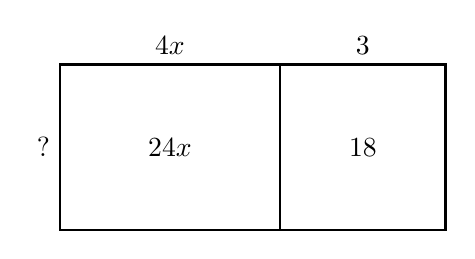
\begin{tikzpicture}[scale=0.7]
  \draw[thick] (0,0) rectangle (7,3);
  \draw[thick] (4,0) -- (4,3);
  \node[left] at (0,1.5) {?};
  \node[above] at (2,3) {$4x$};
  \node[above] at (5.5,3) {$3$};
  \node at (2,1.5) {$24x$};
  \node at (5.5,1.5) {$18$};
\end{tikzpicture}
\end{center}
\end{questionText}
\choiceA{$6(4x + 3)$}
\choiceB{$4(6x + 3)$}
\choiceC{$3(8x + 6)$}
\choiceD{$24(x + 18)$}
\correctAnswer{A}
\explanation{The width must satisfy: $? \times 4x = 24x$ and $? \times 3 = 18$. So $? = 6$. The factored form is $6(4x + 3) = 24x + 18$.}
\end{practiceQuestion}

\begin{practiceQuestion}{4-4-q23}{gmc}
\begin{questionText}
The rectangle below has the given area. Which pair of dimensions is correct?

\begin{center}
\begin{tikzpicture}[scale=0.7]
  \draw[thick, fill=funBlue!10] (0,0) rectangle (6,2.5);
  \node at (3,1.25) {Area $= 14x + 21$};
  \node[left] at (0,1.25) {?};
  \node[below] at (3,0) {?};
\end{tikzpicture}
\end{center}
\end{questionText}
\choiceA{Width $= 7$, Length $= 2x + 3$}
\choiceB{Width $= 14$, Length $= x + 21$}
\choiceC{Width $= 7$, Length $= 2x + 21$}
\choiceD{Width $= 3$, Length $= 4x + 7$}
\correctAnswer{A}
\explanation{Factor: $14x + 21 = 7(2x + 3)$. So the width is $7$ and the length is $2x + 3$.}
\end{practiceQuestion}

\begin{practiceQuestion}{4-4-q24}{gmc}
\begin{questionText}
Three expressions are shown below. Which one is the correctly factored form of $15x - 25$?

\begin{center}
\begin{tikzpicture}[scale=0.7]
  % Option boxes
  \node[draw, thick, rounded corners, fill=funBlue!15, minimum width=3.5cm, minimum height=1cm] at (0,0) {A: $3(5x - 25)$};
  \node[draw, thick, rounded corners, fill=funGreen!15, minimum width=3.5cm, minimum height=1cm] at (5.5,0) {B: $5(3x - 5)$};
  \node[draw, thick, rounded corners, fill=funOrange!15, minimum width=3.5cm, minimum height=1cm] at (11,0) {C: $15(x - 25)$};
\end{tikzpicture}
\end{center}
\end{questionText}
\choiceA{A only}
\choiceB{B only}
\choiceC{C only}
\choiceD{A and B}
\correctAnswer{B}
\explanation{GCF of $15$ and $25$ is $5$. Factor: $5(3x - 5)$. Check: $5(3x - 5) = 15x - 25$ \checkmark. Option A: $3(5x - 25) = 15x - 75$ \ding{55}. Option C: $15(x - 25) = 15x - 375$ \ding{55}.}
\end{practiceQuestion}

% --- Graphical Short Answer Questions (3) ---

\begin{practiceQuestion}{4-4-q25}{gsa}
\begin{questionText}
The total area of the two rectangles shown below is $10x + 15$. Both rectangles have the same height $h$. Find the value of $h$.

\begin{center}
\begin{tikzpicture}[scale=0.7]
  \draw[thick, fill=funBlue!15] (0,0) rectangle (4,2.5);
  \node[below] at (2,0) {$2x$};
  \node[left] at (0,1.25) {$h$};
  \draw[thick, fill=funGreen!15] (5,0) rectangle (8,2.5);
  \node[below] at (6.5,0) {$3$};
  \node[right] at (8,1.25) {$h$};
\end{tikzpicture}
\end{center}
\end{questionText}
\correctAnswer{$h = 5$}
\explanation{Total area $= h(2x) + h(3) = h(2x + 3) = 10x + 15$. Factor: $10x + 15 = 5(2x + 3)$. So $h = 5$.}
\end{practiceQuestion}

\begin{practiceQuestion}{4-4-q26}{gsa}
\begin{questionText}
The area model below has one missing product. Find the missing value and write the complete factored expression.

\begin{center}
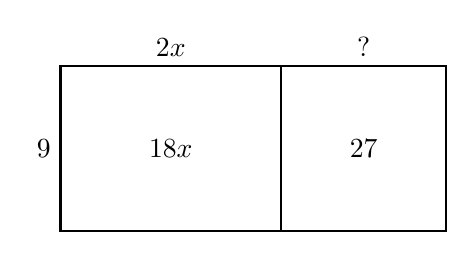
\begin{tikzpicture}[scale=0.7]
  \draw[thick] (0,0) rectangle (7,3);
  \draw[thick] (4,0) -- (4,3);
  \node[left] at (0,1.5) {$9$};
  \node[above] at (2,3) {$2x$};
  \node[above] at (5.5,3) {$?$};
  \node at (2,1.5) {$18x$};
  \node at (5.5,1.5) {$27$};
\end{tikzpicture}
\end{center}
\end{questionText}
\correctAnswer{Missing value is $3$; factored expression: $9(2x + 3) = 18x + 27$}
\explanation{$9 \times ? = 27$, so $? = 3$. The factored expression is $9(2x + 3)$. Check: $9(2x + 3) = 18x + 27$ \checkmark.}
\end{practiceQuestion}

\begin{practiceQuestion}{4-4-q27}{gsa}
\begin{questionText}
A bakery sells boxes of cookies. The sign shows the pricing. Write the total cost for $n$ boxes as a product of the GCF and a sum, then expand to verify.

\begin{center}
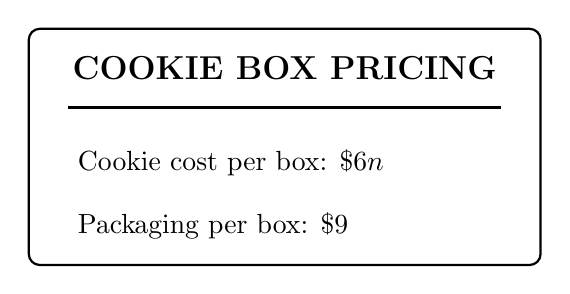
\begin{tikzpicture}
  \draw[thick, rounded corners] (0,0) rectangle (6.5,3);
  \node[font=\bfseries\large] at (3.25,2.5) {COOKIE BOX PRICING};
  \draw[thick] (0.5,2) -- (6,2);
  \node[align=left, anchor=west] at (0.5,1.3) {Cookie cost per box: $\$6n$};
  \node[align=left, anchor=west] at (0.5,0.5) {Packaging per box: $\$9$};
\end{tikzpicture}
\end{center}
\end{questionText}
\correctAnswer{$3(2n + 3)$; expands to $6n + 9$}
\explanation{Total cost: $6n + 9$. GCF of $6$ and $9$ is $3$. Factor: $3(2n + 3)$. Check: $3(2n + 3) = 6n + 9$ \checkmark.}
\end{practiceQuestion}
